\documentclass{article}
\usepackage[a4paper, margin = 1.7cm]{geometry}
\usepackage[english]{babel}
\usepackage{float}
\usepackage{graphicx}
\usepackage{gensymb}
\usepackage{csquotes}
\usepackage{hyperref}

\title{Pseudo code for mobile robot}
\author{Lennart Großkreutz}
\date{\today}

\usepackage{algorithm2e}

\begin{document}

\maketitle

\section{Definitions}
We use the term \textit{center line} to describe the line depicted in the graphic below: \\
\hspace{10mm}

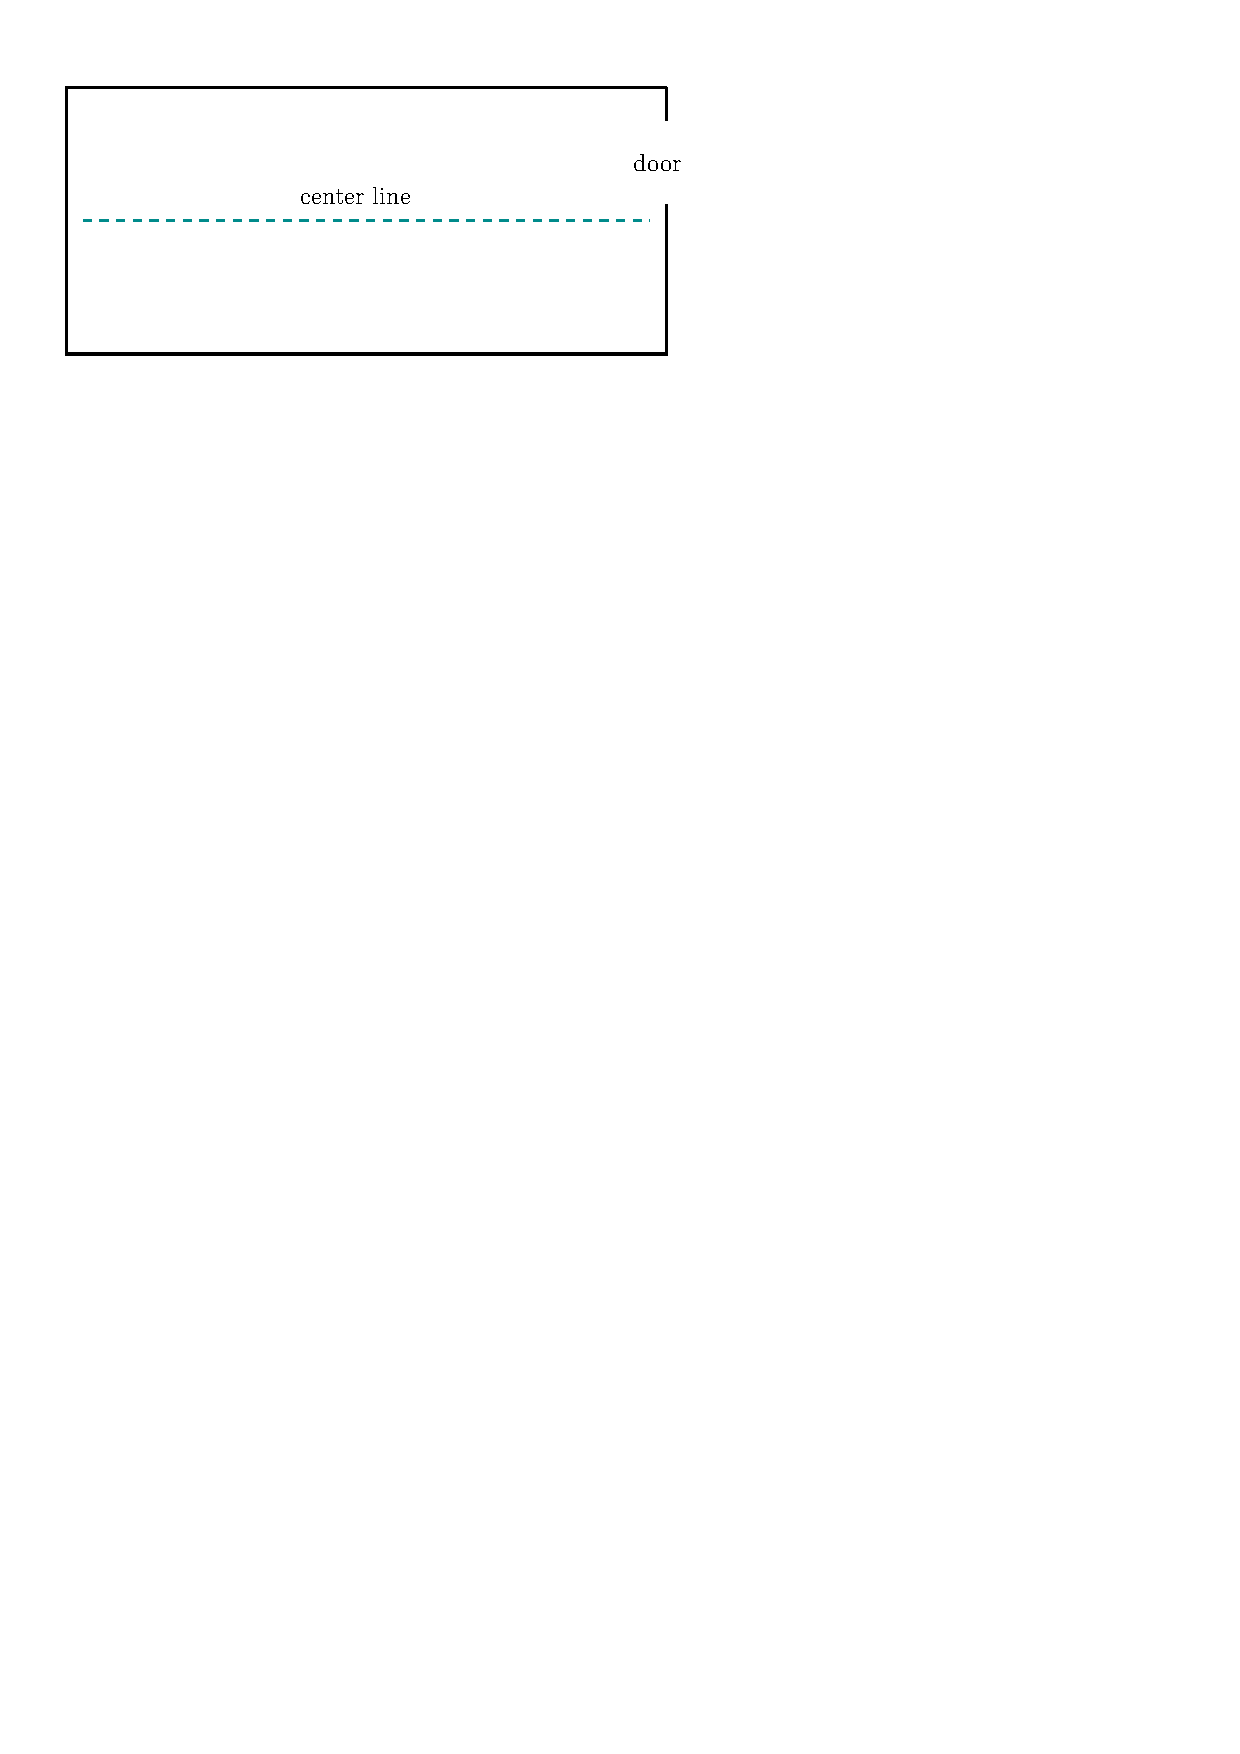
\includegraphics[width=.6\textwidth]{images/center-line.pdf}

\section{Algorithm}
\begin{algorithm}[H]
	%\DontPrintSemicolon
	\KwData{none}
	\KwResult{robot leaves the room through the open door without touching any obstacles}
	\BlankLine
	\While{door not yet passed}{
		measurements $\longleftarrow$ scan()\;
		\uIf{the two long parallel walls detected in measurements}{
			\uIf{robot not on the center line yet}{
				rotate so that center line is in sight with no obstacles in between\;
				move a fixed distance $d_{searching}$ towards center line\;
			}
			\uElse(\tcp*[f]{robot already on center line}){
				\uIf{robot's gaze direction not aligned with center line}{
					rotate the shorter way until robot's gaze is aligned with center line\;
				}
				\uIf{distance from robot to wall $\leq$ fixed distance $d_{wall}$} {
					\tcp{$\alpha, \beta$ are constants indicating in which angle range to search the door}	
					(doorDetected, doorMiddleAngle) = detectDoorInAngleRange($\alpha, \beta$)\;
					\uIf{doorDetected}{
						\tcp{Hope to pass the door now}
						rotate so that robot is facing in the direction of doorMiddleAngle\;
						move forward a fixed distance $d_{door}$\;
						return\; 
					}
					\uElse{
						\tcp{door wasn't found on this site of the center line, turn}
						rotate so that robot's gaze is aligned with center line in other direction\;
					}
				}
				move forward a fixed distance $d_{centerline}$
			}
			
		}
		\uElse(\tcp*[f]{no clue where robot is in the room}){
			\While{nearby obstacle in gaze direction}
			{rotate by a random angle in a fixed range $[ \alpha, \beta]$}
		}
		move forward a fixed distance $d_{random}$
	}
	\caption{Room escape}
\end{algorithm}

\section{Sub-Routines} 
In this section, sub-routines are described semantically.

\subsection{Sub-Routine \textit{scan()}}
The robot gradually does a full rotation, meanwhile creating a list of measurements. 
It stores the current distance captured by the sensor, then it rotates for a fixed angle
$\phi$ (e.g. $\phi = 1 \degree$) until the robot has completed a full rotation.
$\phi$ should be chosen as divider of $2 \pi = 360 \degree$ so that the robot returns to the original gaze direction after the scan.

\subsection{Sub-Routine \textit{detectDoorInAngleRange($\alpha, \beta$)}}
This sub-routine does a partial scan in the angle range determined by the function arguments
$\alpha$ and $\beta$. 
If a considerable and sudden increase in distance values followed by a considerable and sudden decrease is 
detected within this partial scan, we interpret this as the door and output the estimated angle corresponding to the vertical door middle as well.
 
The core idea is that this function is only called when we already have some information about 
the robot's position, namely that it's on the center line and that its gaze direction is aligned
with the center line and it's close to a wall in sight.
These information enable us to search for the port in a certain angle range.
In a previous version of the algorithm, we searched for a door-like pattern in the distance array of an entire rotation.
This led to problems because table legs also produce door-like patterns in the distance array, so the area between two table legs was often misinterpreted as the real door.

\section{Technical remarks}
The robot does never know certainly whether it passed the door, so the outer loop is rather \enquote{while(true)}. The robot is stopped externally as soon as it passed the door.
That's also why the \textit{return;} statement doesn't appear in the real code.

\section{Simulation}
Parallel to the development of the algorithm, we wrote a simulation in Python using Pygame.
The simulation allows us to build a model of the room and to test different ideas for algorithms.
The robot in the simulation uses differential drive kinematics and is equipped with a laser sensor.
We chose a laser sensor because it was easier to implement than an ultrasonic sensor,
however we hope that this doesn't much impact the algorithm's success.
One can also limit the range of the laser sensor.
While we are not able to \textit{prove} that an algorithm will work on the real robot just by
demonstrating its good performance in the simulation, the simulation served another purpose:
If an idea is not even working in the simulated environment with perfect sensor data,
and won't work on the robot as well.

A screenshot of the simulation is visible in Figure \ref{fig:sim}.
The source code can be found on Github: \url{https://github.com/LennartGr/Differential-Drive-Robot-with-Pygame}.

\begin{figure}[b]
	\centering
	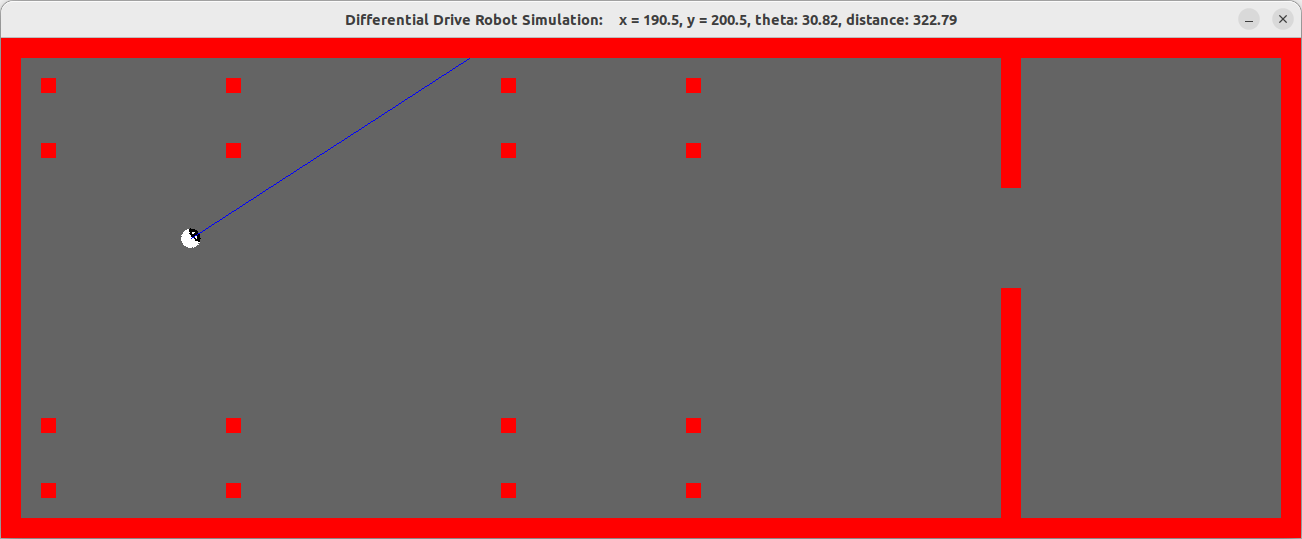
\includegraphics[width=.95\textwidth]{images/simulation.png}
	\caption{Simulation using Pygame}
	\label{fig:sim}
\end{figure}

\end{document}